\label{sec:usecases}
This section describes the use cases of the system. These use cases only cover the basics like creating and managing events and responding to event invites.

A more complete, real-world system could benefit from additions as:
\begin{itemize}
	\item a comment system that allows people to discuss event details.
	\item a richer environment for event organizers that includes a picture gallery.
	\item a notification system on the website.
	\item integration with event features from popular social networks.
	\item more options for inviting people (for instance, allow invitees to invite new people for public events).
	\item allowing closed events to be reopened (and in general a more flexible event system).
\end{itemize}
\subsection{Use Case Diagram}
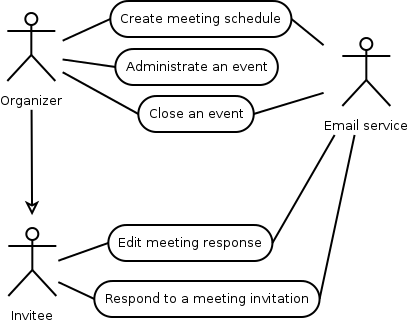
\includegraphics{ucd/ucd.png}
\pagebreak
\subsection{Create meeting schedule}

\begin{description}
	\item[Pre-condition:] User is registered and logged in
	\item[Trigger:] User clicks 'Schedule new event' link
	\item[Guarantee:] A new event is created
	\item[Scenarios]\textbf{:}\\
				\begin{description}
					\item[Main scenarios]\textbf{:}\\
								\begin{enumerate}
									\item The user enters his/her name, the event name and an event description.
									\item The user enters some date/time options.
									\item The user enters email addresses for attendees and a custom message.
									\item The user specifies whether or not the poll should be 'hidden' and voting limitations.
									\item The user submits the event to the system by opening the poll.
									\item The system sends confirmation and invitation emails.
								\end{enumerate}
					\item[Alternatives]\textbf{:}\\
								\begin{itemize}
									\item 2.1 One or more date/time pairs are not valid, the system shows an error message and the user is back at the start of step 2, with all fields already filled in, except for the invalid ones.
								\end{itemize}
				\end{description}
\end{description}
\pagebreak

\subsection{Respond to a meeting invitation}

\begin{description}
	\item[Pre-condition:] User has received an invitation email and the meeting poll is open
	\item[Trigger:] User clicks the link in the invitation email
	\item[Guarantee:] The user voted on possible dates
	\item[Scenarios]\textbf{:}\\
				\begin{description}
					\item[Main scenarios]\textbf{:}\\
								\begin{enumerate}
									\item The user confirms that he or she would like to attend the event.
									\item The user votes on date/time options.
									\item The system sends a notification email to the organizer.
									\item The user is able to see the votes of other invitees.
								\end{enumerate}
					\item[Alternatives]\textbf{:}\\
								\begin{itemize}
									%TODO: Not sure if an alternative is really the way to go. I used to have a seperate use case for accepting and declining, but that seemed a bit superfluous.
									\item 1.1 If the user doesn't want to participate in the event, he or she declines the invitation.	The use case is ended
									\item 2.1 If the organizer made any voting restrictions, such as enabling users to only vote once or limiting the number of invitees that can vote on a certain date/time, these are enforced. They will continue to step 3.
									\item 4.1 If the poll was marked 'hidden' by the organizer, the results are not shown. The use case is ended.
								\end{itemize}
				\end{description}
\end{description}
\pagebreak
\subsection{Edit a meeting response}

\begin{description}
	\item[Pre-condition:] User has responded to a meeting invitation and the meeting poll is open
	\item[Trigger:] User clicks the link in the invitation email
	\item[Guarantee:] The users can confirm his presence by answering the poll.
	\item[Scenarios]\textbf{:}\\
				\begin{description}
					\item[Main scenarios]\textbf{:}\\
								\begin{enumerate}
									\item The user confirms that he/she would still like to attend the event.
									\item The user votes on date/time options.
									\item The system sends a notification email to the organizer.
									\item The user is able to see the votes of other invitees.
								\end{enumerate}
					\item[Alternatives]\textbf{:}\\
								\begin{itemize}
									\item 1.1 If the user doesn't want to participate anymore, he or she can decide to decline the invitation. The use case is ended
									\item 4.1 If the poll was marked 'hidden' by the organizer, the results are not shown. The use case is ended.
								\end{itemize}
				\end{description}
\end{description}


\subsection{Administrate an event}

\begin{description}
	\item[Pre-condition:] The user is the organizer for this event
	\item[Trigger:] User clicks the link to administrate the event
	\item[Guarantee:] Settings for the event might have changed
	\item[Scenarios]\textbf{:}\\
				\begin{description}
					\item[Main scenarios]\textbf{:}\\
								\begin{enumerate}
									\item The user is presented with an overview of the event.
									\item The user chooses to delete the event, edit the general settings, change the date/time options or view event logs.
								\end{enumerate}
				\end{description}
\end{description}
\pagebreak
\subsection{Close an event}

\begin{description}
	\item[Pre-condition:] The user is the organizer for this event
	\item[Trigger:] User clicks the link to administrate the event and then clicks the delete button
	\item[Guarantee:] The event is closed
	\item[Scenarios]\textbf{:}\\
				\begin{description}
					\item[Main scenarios]\textbf{:}\\
								\begin{enumerate}
									\item The system let user confirms his choice.
									\item The user selects the final date/time based on the poll results.
									\item Optionally, the user enters a closing message for the event.
									\item An email containing the optional message and the final date/time is sent to each invitee that confirmed.
									\item The event is closed.
								\end{enumerate}
					\item[Alternatives]\textbf{:}\\
								\begin{itemize}
									\item 1.1 If the user clicks 'no', the closing is cancelled. The use case is ended.
								\end{itemize}
					\item[Design decision]\textbf{:}\\Wewant to confirm the choice because when the event is deleted there is no way back and it will cancel the whole event.
				\end{description}
\end{description}

